\documentclass[xcolor={table,usenames,dvipsnames}]{beamer}
\setbeamercovered{transparent}
\usepackage{stackengine}
\usepackage{scalerel}
\usepackage{eso-pic} 
\newcommand\dangersign[1][2ex]{%
  \renewcommand\stacktype{L}%
  \scaleto{\stackon[1.3pt]{\color{red}$\triangle$}{\tiny !}}{#1}%
}
\usepackage[absolute,overlay]{textpos}
\usepackage{colortbl}
\usepackage{array}
\usepackage{fourier}
\usepackage{booktabs}% http://ctan.org/pkg/booktabs
\newcommand{\tabitem}{~~\llap{\textbullet}~~}

\usepackage{tabularx}
\setbeamertemplate{blocks}[rounded][shadow=true]
%\let\olditem\item
%\renewcommand{\item}{%
%\olditem\vspace{0pt}}   
  
\usepackage{ragged2e}

%\usepackage[round]{natbib} % incompatible avec biblatex
\usepackage{hyperref}
\hypersetup{
    colorlinks=true,
    linkcolor=.,
    filecolor=deepblue,      
    urlcolor=deepblue,
    pdftitle={Overleaf Example},
    pdfpagemode=FullScreen,
    citecolor=deepblue
    }
\definecolor{LightCyan}{rgb}{0.88,1,1}   
\usepackage[justification=centering,size=scriptsize]{caption}
\usepackage[size=footnotesize]{subcaption}
\captionsetup{font=scriptsize}
\captionsetup[figure]{name=Fig.}
\setbeamertemplate{caption}[numbered]
\usepackage[T1]{fontenc}
\usepackage{ctex}
\UseRawInputEncoding
%\usepackage[backend=bibtex, style=authoryear, natbib=true, sorting=nty, backref=true]{biblatex}
\usepackage[style=authoryear, maxbibnames=99, mincitenames=1, maxcitenames=2, backref=true, hyperref=true, dashed=false, firstinits=true, backend=bibtex, bibencoding=utf8, uniquename=false, uniquelist=false, natbib=true]{biblatex}
\renewcommand*{\bibfont}{\footnotesize}

% Remove quotation marks from titles
\DeclareFieldFormat[article,incollection,inproceedings,conference]{title}{#1} 
\addbibresource{ref.bib}

%\usepackage[backend=bibtex,
%style=authoryear,
%natbib=true,
%sorting=nty,
%backref=true
%]{biblatex}

\let\oldnocite\nocite
\makeatletter
\renewcommand*{\nocite}[1]{\oldnocite{#1}\Hy@backout{#1}}
\makeatother

\renewcommand*{\bibfont}{\footnotesize}

\DeclareCiteCommand{\cite}
  {\usebibmacro{prenote}}
  {\usebibmacro{citeindex}%
   \printtext[bibhyperref]{\usebibmacro{cite}}}
  {\multicitedelim}
  {\usebibmacro{postnote}}

\DeclareCiteCommand*{\cite}
  {\usebibmacro{prenote}}
  {\usebibmacro{citeindex}%
   \printtext[bibhyperref]{\usebibmacro{citeyear}}}
  {\multicitedelim}
  {\usebibmacro{postnote}}

\DeclareCiteCommand{\parencite}[\mkbibparens]
  {\usebibmacro{prenote}}
  {\usebibmacro{citeindex}%
    \printtext[bibhyperref]{\usebibmacro{cite}}}
  {\multicitedelim}
  {\usebibmacro{postnote}}

\DeclareCiteCommand*{\parencite}[\mkbibparens]
  {\usebibmacro{prenote}}
  {\usebibmacro{citeindex}%
    \printtext[bibhyperref]{\usebibmacro{citeyear}}}
  {\multicitedelim}
  {\usebibmacro{postnote}}

\DeclareCiteCommand{\footcite}[\mkbibfootnote]
  {\usebibmacro{prenote}}
  {\usebibmacro{citeindex}%
  \printtext[bibhyperref]{ \usebibmacro{cite}}}
  {\multicitedelim}
  {\usebibmacro{postnote}}

\DeclareCiteCommand{\footcitetext}[\mkbibfootnotetext]
  {\usebibmacro{prenote}}
  {\usebibmacro{citeindex}%
   \printtext[bibhyperref]{\usebibmacro{cite}}}
  {\multicitedelim}
  {\usebibmacro{postnote}}

%\DeclareCiteCommand{\textcite}
%  {\boolfalse{cbx:parens}}
%  {\usebibmacro{citeindex}%
%   \printtext[bibhyperref]{\usebibmacro{textcite}}}
%  {\ifbool{cbx:parens}
%     {\bibcloseparen\global\boolfalse{cbx:parens}}
%     {}%
%   \multicitedelim}
%  {\usebibmacro{textcite:postnote}}

        \DeclareCiteCommand{\textcite}
        {\usebibmacro{cite:init}%
            \usebibmacro{prenote}}
        {\usebibmacro{citeindex}%
            \printtext[bibhyperref]{\usebibmacro{textcite}}}
        {}
        {\printtext[bibhyperref]{\usebibmacro{textcite:postnote}}%
            \usebibmacro{cite:post}}

\addbibresource{ref.bib}

% Cannot enable in Xelatex
\usepackage{pgfpages}
% \setbeameroption{hide notes} % Only slides
% \setbeameroption{show only notes} % Only notes
% \setbeameroption{show notes on second screen}

% other packages
\usepackage{latexsym,amsmath,multicol,booktabs,calligra}
\usepackage{graphicx,listings,stackengine}
\usepackage[greek,french]{babel}
\usepackage[LGR,T1]{fontenc}
\usepackage{fontspec}

%\usepackage[sfdefault,light,scaled=.85]{merriweather} %% Option 'black' gives heavier bold face 


\usepackage[sfdefault]{AlegreyaSans} %% Option 'black' gives heavier bold face
%% The 'sfdefault' option to make the base font sans serif
\renewcommand*\oldstylenums[1]{{\AlegreyaSansOsF #1}}



% Define a command for text in Greek. Replace 'Gentium Plus' with a font of your choice if necessary.
\newfontfamily\greekfont{Gentium Plus}
\newcommand{\textgreek}[1]{{\greekfont #1}}

\DefineBibliographyStrings{french}{%
  backrefpage = {voir p\adddot},%
  backrefpages = {voir pp\adddot}%
}
\DeclareFieldFormat{pagerefformat}{\mkbibparens{{\color{red}\mkbibemph{#1}}}}
\renewbibmacro*{pageref}{%
  \iflistundef{pageref}
    {}
    {\printtext[pagerefformat]{%
       \ifnumgreater{\value{pageref}}{1}
         {\bibstring{backrefpages}\ppspace}
         {\bibstring{backrefpage}\ppspace}%
       \printlist[pageref][-\value{listtotal}]{pageref}}}}
\usepackage{wasysym}
% Enable only in Xelatex
 \usepackage{pstricks}

\author[Ljudmila PETKOVIC]{\small \textbf{Ljudmila PETKOVIC}\textsuperscript{1,2,3}\\\medskip{\footnotesize\texttt{prenom.nom@sorbonne-universite.fr}}}
\title[Extraction des concepts-clés à partir du fonds Charcot]{\fontsize{13pt}{13pt}\selectfont Extraction des concepts-clés à partir du fonds Charcot}
\subtitle{Approche \textit{PatternRank}}
\institute [JE \og{}Humanités numériques\fg{}] {\tiny \textsuperscript{1} Sorbonne Université, Faculté des Lettres, \textsc{UFR} Littératures françaises et comparée, ED 3\\\textsuperscript{2} Centre d'étude de la langue et des littératures françaises (\textsc{CELLF}), \textsc{UMR 8599}\\\textsuperscript{3} Observatoire des textes, des idées et des corpus (\textsc{ObTIC})}
\date[DataLab, le 30 avril 2024]{\scriptsize  Atelier \textsc{ObTIC}\\DataLab, \textsc{BnF}\\Paris, le 30 avril 2024}
\usepackage{YTU}

% defs
\def\cmd#1{\texttt{\color{red}\footnotesize $\backslash$#1}}
\def\env#1{\texttt{\color{blue}\footnotesize #1}}
\definecolor{deepblue}{rgb}{0,0,0.5}
\definecolor{deepred}{rgb}{0.6,0,0}
\definecolor{deepgreen}{rgb}{0,0.5,0}
\definecolor{halfgray}{gray}{0.55}
\definecolor{warmblack}{rgb}{0.0, 0.26, 0.26}

\lstset{
    basicstyle=\ttfamily\small,
    keywordstyle=\bfseries\color{deepblue},
    emphstyle=\ttfamily\color{deepred},    % Custom highlighting style
    stringstyle=\color{deepgreen},
    numbers=left,
    numberstyle=\small\color{halfgray},
    rulesepcolor=\color{red!20!green!20!blue!20},
    frame=shadowbox,
}
% \logo{%
%     
\includegraphics[width=1cm,height=1cm,keepaspectratio]{pic/obtic.jpg}~%
%     
\includegraphics[width=1cm,height=1cm,keepaspectratio]{pic/Lettres_su_logo.png}~%
% }
\usepackage{enumerate}
\setbeamertemplate{section in toc}{\hspace*{1em}\inserttocsectionnumber.~\inserttocsection\par}
\setbeamertemplate{subsection in toc}{\hspace*{2em}\inserttocsectionnumber.\inserttocsubsectionnumber.~\inserttocsubsection\par}
\renewcommand*{\bibfont}{\scriptsize}



\let\oldfootnotesize\footnotesize
\renewcommand*{\footnotesize}{\oldfootnotesize\scriptsize}

%\setbeamertemplate{itemize/enumerate body begin}{\small}
\setbeamertemplate{itemize/enumerate subbody begin}{\small}
%
%\newcommand{\leftquote}{{\fontfamily{lmr}\selectfont\textquotedblleft}}
%\newcommand{\rightquote}{{\fontfamily{lmr}\selectfont\textquotedblright}}
%\newcommand{\leftguillemet}{{\fontfamily{lmr}\selectfont\guillemotleft}}
%\newcommand{\rightguillemet}{{\fontfamily{lmr}\selectfont\guillemotright}}





\begin{document}

\begin{frame}
    \titlepage
\begin{figure}
    \centering
    
    
\includegraphics[width=2cm,height=1cm,keepaspectratio]{pic/Lettres_su_logo.png}~\hspace*{0.5cm}%\includegraphics{}
    
\includegraphics[width=2cm,height=1cm,keepaspectratio]{pic/cellf.png}~\hspace*{0.5cm}%
    
\includegraphics[width=3cm,height=1cm,keepaspectratio]{pic/obtic.jpg}~%

\end{figure}
    
    \begin{note}
        {Introduce your self}
    \end{note}

\end{frame}

\begin{frame}
\frametitle{Plan}
    \tableofcontents[sectionstyle=show,subsectionstyle=show/shaded/hide,subsubsectionstyle=show/shaded/hide]
\end{frame}

%\section[Contexte]{Contexte de recherche}
%\subsection{Rupture épistémologique}
%\begin{frame}{\og{}Napoléon des névroses\fg{} ou \og{}Paganini de l'hystérie\fg{} {\small(\hypersetup{citecolor=yellow}\cite{marmion2015freud})}}

\textsc{\textcolor{deepblue}{\textbf{Jean-Martin CHARCOT}} (1825-1893)} 
%\hbox{\hspace{25em} 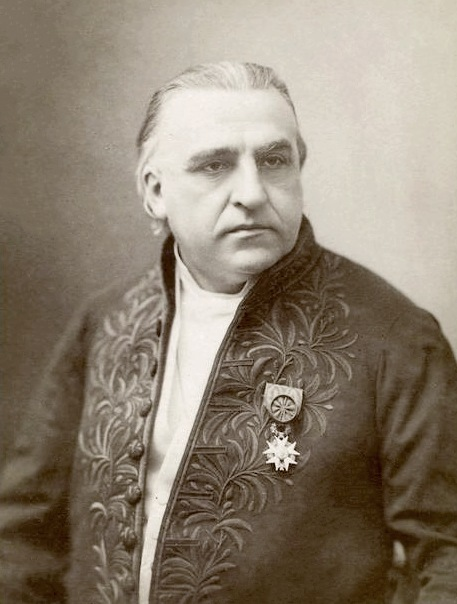
\includegraphics[scale=0.07]{pic/Jean-Martin_Charcot.jpg}}
%\\{\scriptsize Portrait de\\Charcot (\href{https://fr.wikipedia.org/wiki/Jean-Martin_Charcot}{Wikipedia}).}
\hbox{\hspace{10.3em} 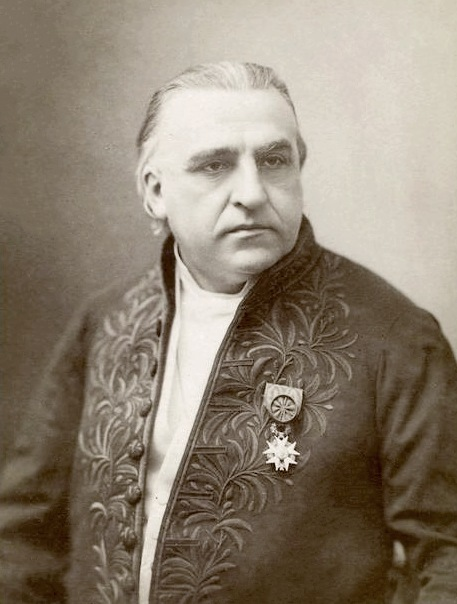
\includegraphics[scale=0.06]{pic/Jean-Martin_Charcot.jpg}}\\\hbox{\hspace{23.8em}{\tiny Source : \href{https://fr.wikipedia.org/wiki/Jean-Martin_Charcot}{Wikipedia}}.} \pause
\begin{itemize}[<+->]
\item père de la neurologie moderne en France au XIX\ieme{} s. 
\item leçons cliniques du mardi à l'hôpital de la Salpêtrière à Paris \\
\hspace{165pt}
\footnotesize\og{}Mecque de la neurologie\fg{}
\end{itemize}

\begin{enumerate}[\indent {}]
\only<4->{\item Contributions majeures:}
\small
    \begin{tabular}{l l}
    \only<5->{\textcolor{darkgray}{hystérie} & $\leftarrow$ lésion dynamique des circuits cérébraux} \\
    \only<6->{\textcolor{darkgray}{hypnose} & analyse et traitement des symptômes hystériques} \\
    \only<7->{\textcolor{darkgray}{SEP} & description de la \textit{sclérose en plaques} disséminée} \\
    \only<8->{\textcolor{darkgray}{SLA} & description de la \textit{sclérose latérale amyotrophique}} \\
    \only<9->{\textcolor{darkgray}{maladie de Parkinson} & concepteur du terme (avec A. Vulpian)} \\
    \end{tabular}
\end{enumerate}
%\begin{itemize}[<+->]
%\small
%\item[] \textcolor{darkgray}{hystérie} & $\leftarrow$ lésion dynamique des circuits cérébraux 
%\item[] \textcolor{darkgray}{hypnose} & analyse et traitement des symptômes hystériques 
%\item[] \textcolor{darkgray}{SEP} & description de la \textit{sclérose en plaques} disséminée 
%\item[] \textcolor{darkgray}{SLA} & description de la \textit{sclérose latérale amyotrophique} 
%\item[] \textcolor{darkgray}{maladie de Parkinson} & concepteur du terme (avec A. Vulpian) 
%\end{itemize}
\pause
%\vspace{-0.3cm} \pause
\begin{flushright}
{\footnotesize(\cite{camargo2024jean})}
\end{flushright}

%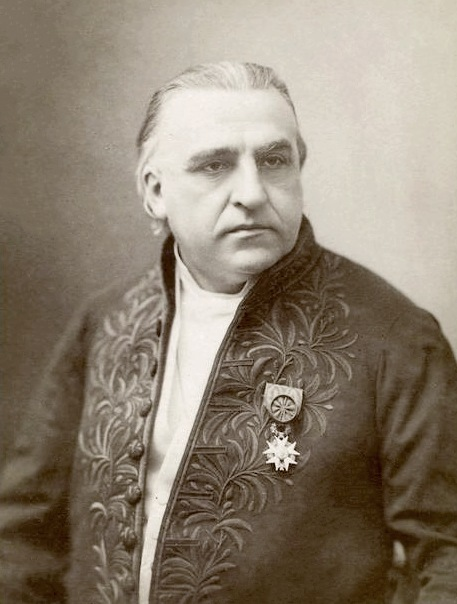
\includegraphics[width=10pt]{pic/Jean-Martin_Charcot.jpg}%
%\\{\scriptsize Portrait de\\Charcot (\href{https://fr.wikipedia.org/wiki/Jean-Martin_Charcot}{Wikipedia}).}
\end{frame}

\begin{frame}{Impact de Charcot sur sa discipline et au-delà}
\centering
\textbf{Collaborateurs et élèves} \pause \\
{\small \og{}réseau scientifique\fg{}} \pause
    \begin{table}[!ht]
        \centering
        \small
        \begin{tabular}{l l r}
           \only<3->{Sigmund \textsc{Freud} & 1856-1939  & théorie psychanalytique} \pause \\
            \only<4->{Gilles \textsc{de la Tourette} & 1857-1932 & syndrôme de Tourette} \pause \\
            \only<5->{Joseph \textsc{Babinski} & 1857-1904 & pithiatisme, signe de Babinski} 
%           Pierre \textsc{Janet} (1859-1947) & psychopathologie
%            dissociation, sous-conscient 
        \end{tabular}
        \pause
        \begin{flushright}
%        \footnotesize\citep{bogousslavsky2020}
        \footnotesize\citep{BROUSSOLLE2012301}
        \end{flushright}
        % \caption{Caption}
        \label{tab:my_label}
    \end{table}
    \pause
\medskip
\textbf{Écrivains naturalistes français et européens} \pause
\begin{itemize}
\centering
\small \item références à Charcot et aux descriptions de crises hystériques
\end{itemize} \pause
\begin{table}[!ht]
    \centering
    \small
    \begin{tabular}{l l r}
        \only<9->{Émile \textsc{Zola} & 1840–1902  & \textit{Lourdes}} \\
        \only<10->{Léon \textsc{Tolstoï} & 1828–1910 & \textit{La Sonate à Kreutzer}} \\
        \only<11->{Luigi \textsc{Capuana} & 1839–1915 & \textit{La Torture}}
%        Bjørnstjerne \textsc{Bjørnson} (1832–1910) & \textit{Over Ævne}
    \end{tabular}
    \pause
    \begin{flushright}
    \footnotesize\citep{koehler2013charcot}
    \end{flushright}
    % \caption{Caption}
    \label{tab:my_label}
\end{table}

\end{frame}

\begin{frame}{Fonds Charcot}
\begin{block}{SorbonNum\\
\footnotesize{Bibliothèque de Sorbonne Université (\textsc{BSU})}}
201 documents XML OCRisés (sans post-correction)
\end{block}
%\begin{itemize}
%    \item \textrm{Charcot} : textes rédigés par Charcot
%    \item \textrm{Autres} : textes rédigés par les membres de son réseau scientifique
%\end{itemize}
\begin{table}[!ht]
    \centering
    \begin{tabular}{|c|r|r|}
    \hline 
    \rowcolor{yellow!30}
       Corpus & \multicolumn{1}{c|}{Nb de docs} & \multicolumn{1}{c|}{Nb de tokens} \\
       \hline
      \begin{tabular}[c]{@{}c@{}}\textrm{Charcot}\\ \scriptsize{textes rédigés par Charcot}\end{tabular}  & 68 & 12 190 649 (38,12\%) \\
       \hline
       \begin{tabular}[c]{@{}c@{}}\textrm{Autres}\\ \scriptsize{textes rédigés par les membres} \vspace{-0.15cm} \\ \scriptsize{de son réseau scientifique}\end{tabular}    & 133 & 19 788 830 (61,88\%) \\
       \hline\hline
       \textbf{Total} & \textbf{201} & \textbf{31 979 479} (100\%)\\
       \hline
    \end{tabular}
    \caption{Répartition du corpus issu du \href{https://patrimoine.sorbonne-universite.fr/collection/Fonds-Charcot}{fonds Charcot}.
%    \footnote{\tiny{\url{https://patrimoine.sorbonne-universite.fr/collection/Fonds-Charcot}}}
}
    \label{tab:my_label}
\end{table}
\end{frame}

%\begin{frame}{Corpus Charcot \href{https://obtic.huma-num.fr/obvie/charcot/?view=corpus}{\textcolor{yellow}{en ligne}}}
%Corpus Charcot accessible sur la plateforme \textsc{OBVIE} \hfill {\small\citep{alrahabi2022obvie}}
%\begin{itemize}
%\item fouille avancée des corpus en \textsc{XML-TEI}
%\item textes similaires : mots fréquents / en commun, noms cités
%\end{itemize}
%%\danger impossible de quantifier l'importance des MWEs
%\begin{figure}[!h]
%    \centering
%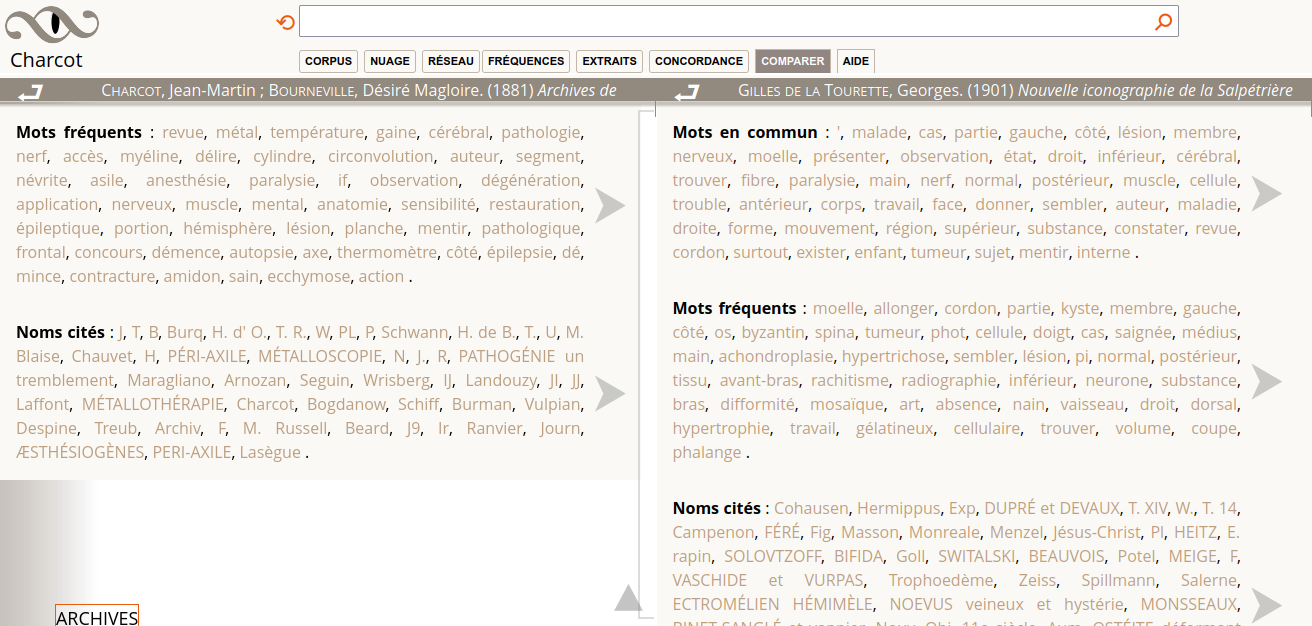
\includegraphics[width=90mm,scale=0.5]{pic/doc_sim.png}
%    \caption{Points similaires entre un ouvrage de Charcot et de celui de de la Tourette.}
%%    \caption{Distribution des fréquences des tokens avec la frise chronologique pour ceux constituant l'expression \textit{bulbe rachidien} (issus des corpus \og{}Charcot\fg{} et \og{}Autres\fg{}).}
%    \label{fig:my_label}
%\end{figure}
%% citations directes (\cite{manjavacas2019})
%\end{frame}

\begin{frame}{Mesurer le degré d'intertextualité}
Mesurer informatiquement l'impact de Charcot sur son réseau \\$\rightarrow$ intertextualité uni-directionnelle
\begin{figure}[!h]
    \centering
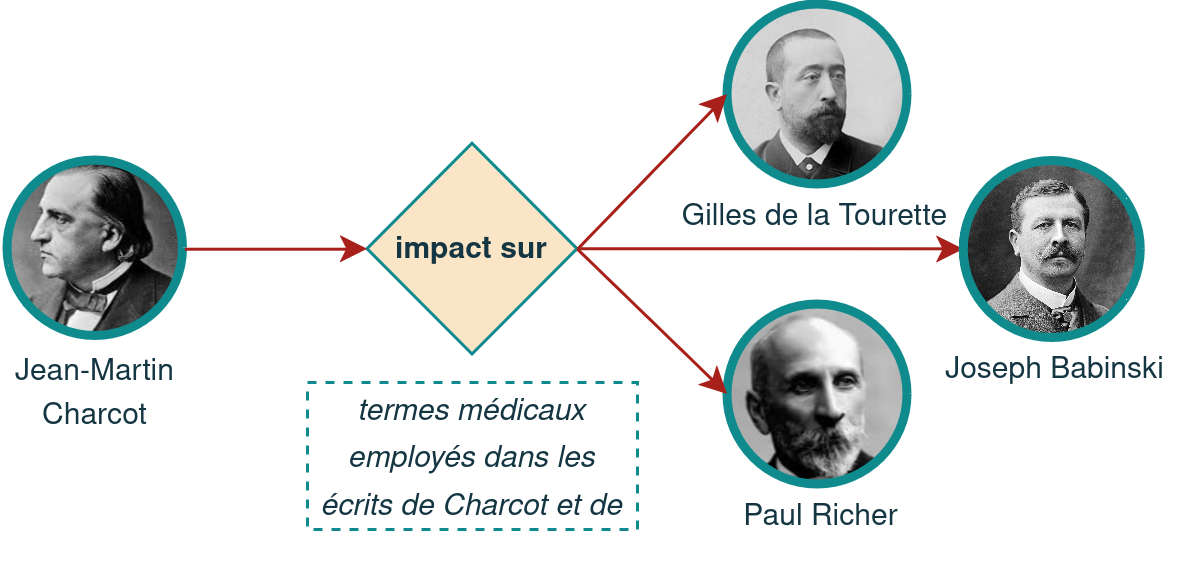
\includegraphics[width=90mm,scale=0.5]{pic/charcot_intertextualite.png}
    \caption{Opérationnalisation de l'impact de Charcot sur ses élèves.}
    \label{fig:my_label}
\end{figure}
\end{frame}

\begin{frame}{Question de recherche}
% Comment mesurer le degré d'intertextualité entre Charcot et son réseau scientifique et artistique au prisme du numérique ?
% create the main block
%\begin{exampleblock}{}
%\centering
%    \color{deepblue}{\textmd{Comment mesurer le degré d'intertextualité entre Charcot et son réseau scientifique au prisme du numérique ?}}
%\end{exampleblock}

\begin{exampleblock}{}
\centering
    \color{deepblue}{\textmd{Peut-on repérer les concepts-clés communs aux discours de Charcot et de son réseau scientifique ?}}
\end{exampleblock}
\end{frame}

%\section[État de l'art]{Extraction des phrases-clés : état de l'art}
%\begin{frame}{Définitions de la tâche}
\pause
\centering
Extraction de \og{}\textbf{phrases-clés}\fg{} (angl. \textit{keyphrases})  \pause
\begin{itemize}[<+->]
\item séquences de plusieurs mots (ex. \textit{sclérose latérale amyotrophique})
\item reflètent plus précisément le contexte sémantique du texte \\\small{$\neq$ mots-clés : unigrammes de mot, ex. \textit{sclérose}}
\end{itemize}
\pause
%\begin{block}{Extraction de phrases-clés}
%\justifying
%Processus de \underline{sélection} automatique d'un petit ensemble de phrases les plus pertinentes à partir d'un texte donné \citep{schopf2022}.
%\end{block}
%\begin{block}{Prédiction de phrases-clés}
%\justifying
%Processus de \underline{génération} des phrases-clés qui résument parfaitement un document donné \citep{xie2023}.
\bigskip
\begin{columns}[t,onlytextwidth]
\column{.45\textwidth}
\justifying
\onslide<4->{\textcolor{violet}{Extraction}\hfill
\small
\underline{Sélection} \\
d'un ensemble de phrases les plus pertinentes à partir d'un texte.}
\begin{flushright}
\small{\citep{schopf2022}}
\end{flushright} 
\column{.45\textwidth}
\onslide<5->{\textcolor{violet}{Prédiction}\hfill
\justifying
\small
\underline{Génération} \\
des phrases-clés qui résument parfaitement un document donné.}
\begin{flushright}
\small{\citep{xie2023}}
\end{flushright}
\end{columns}
\end{frame}

\begin{frame}{Approches classiques\\ {\small(\hypersetup{citecolor=yellow}\cite{garaudclassiques})}}
\setbeamercolor{block title}{use=structure,fg=red!50!black,bg=yellow!40}
\setbeamercolor{block body}{use=structure,fg=black,bg=white!20!white}
\pause
\onslide<1->{\begin{block}{\textsc{Statistiques}}
\justifying
Basées sur les fréquences des mots / groupe de mots et leur cooccurrence.
\end{block}}
\pause
\begin{itemize}[<+->]
\small
\item \textsc{TF-IDF} -- \textit{Term Frequency $\cdot$ Inverse Document Frequency} \hfill \citep{sparck1972statistical}
\item \textsc{RAKE} -- \textit{Rapid Automatic Keyword Extraction} \hfill \citep{rose2010automatic}
\item \textsc{YAKE} -- \textit{Yet Another Keyword Extractor} \hfill \citep{CAMPOS2020257}
\end{itemize}

\onslide<6->{\begin{block}{\textsc{Graphes}}
\justifying
Chaque nœud = mot / groupe de mots ; \\chaque arc = probabilité (ou la fréquence) d’observer ces mots ensemble.
\end{block}}
\pause
\begin{itemize}[<+->]
\small
\item SingleRank \hfill \citep{wan2008}
\item TextRank \hfill \citep{mihalcea2004}
\item TopicRank \hfill \citep{bougouin2013topicrank}
\end{itemize}

\end{frame}

\begin{frame}{Approches sémantiques\\ {\small(\hypersetup{citecolor=yellow}\cite{garaudsemantiques})}}
\justifying
%Lier des mots sémantiquement proches et en extraire ceux qui apportent l’information la plus pertinente à l'aide des réseaux de neurones.
\setbeamercolor{block body}{use=structure,fg=black,bg=white!20!white}
\pause
\onslide<1->{\begin{block}{\textsc{Plongements de mots}}
\justifying
Représentent l’ensemble des mots d’un vocabulaire sous forme de vecteurs. Distance entre ces vecteurs $\rightarrow$ mots sémantiquement proches.
%\begin{itemize}
%\item représentation vectorielle de l’ensemble des mots d’un vocabulaire 
%\item distance entre ces vecteurs $\rightarrow$ mots sémantiquement proches
%\end{itemize}
\end{block}}
\pause
\begin{itemize}[<+->]
\item \small{\texttt{fastTextRank}\footnote{\url{https://github.com/jeekim/fasttextrank}}}
\end{itemize}

%\colorbox{yellow!40}{\color{red!50!black}{Plongements de mots}}
%%\textsc{\textit{word2vec}}} \small{\citep{mikolov2013efficient}}}
%\begin{itemize}
%\small
%%\item réseaux de neurones artificiels \og{}simples\fg{}
%\item représentation vectorielle de l’ensemble des mots d’un vocabulaire
%\item distance entre ces vecteurs $\rightarrow$ mots sémantiquement proches
%\item ex. : \texttt{fastTextRank}\footnote{\url{https://github.com/jeekim/fasttextrank}}
%\end{itemize}
\medskip

\setbeamercolor{block body}{use=structure,fg=black,bg=white!20!white}
\pause
\onslide<4->{\begin{block}{\textsc{Plongements contextuels}}
\justifying
Basés sur les modèles de langue pré-entraînés.\\
Gèrent mieux des cas ambiguës (homographes).
%\begin{itemize}
%\item basés sur les modèles de langue pré-entraînés 
%\item gestion des cas ambiguës (homographes)
%\end{itemize}
\end{block}}
\pause
\begin{itemize}[<+->]
\item \small{Key2Vec \hfill \citep{mahata2018key2vec}}
\item \small{Key\textsc{BERT}} \hfill \small{\citep{grootendorst2020keybert}}
\end{itemize}
%\colorbox{yellow!40}{\color{red!50!black}{Plongements contextuels}}
%\begin{itemize}
%\small
%%\item réseaux de neurones artificiels \og{}profonds\fg{} (angl. \textit{deep learning})
%\item basés sur les modèles de langue pré-entraînés
%\item prise en compte du contexte pour mieux capturer la sémantique du texte
%%\item architecture gourmande en temps de calcul et en volume de données
%\item ex. : Key2Vec \citep{mahata2018key2vec}, Key\textsc{BERT} \small{\citep{grootendorst2020keybert}}
%\end{itemize}
\end{frame}

%\begin{frame}{Approches exploitant les modèles de langue -- \texttt{keybert}}
%\justifying
%Librairie Python qui exploite les plongements \textsc{BERT} et la similarité cosinus pour générer les mots/phrases-clés les plus similaires à un document.
%\end{frame}

%\section[\texttt{keybert}]{Méthode \texttt{keybert}}
\begin{frame}{Fonctionnement de la librairie \texttt{keybert}}
\begin{enumerate}
\item entrée : un document
\item tokénisation du document en mots/phrases-clés candidates
\item génération des plongements du document et des mots/phrases-clés
\item calcul de la similarité cosinus document : mots/phrases-clés
\end{enumerate}
\begin{figure}
    \centering
    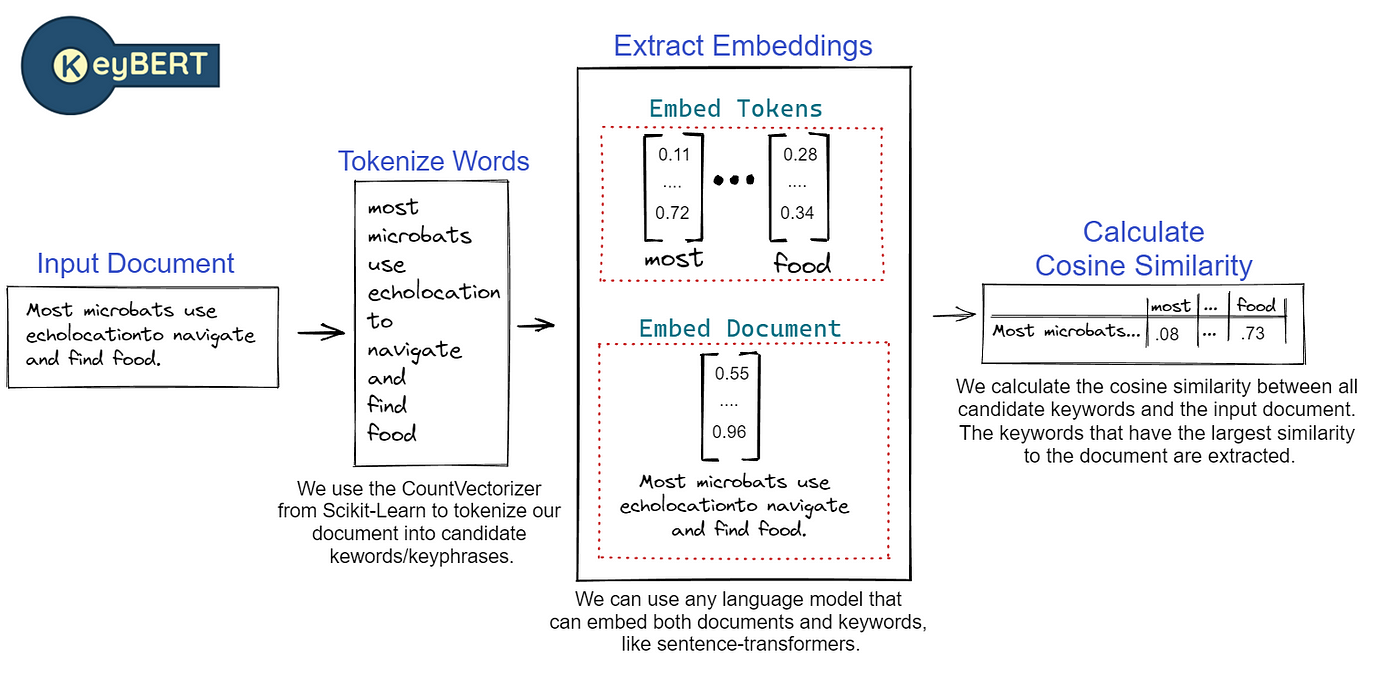
\includegraphics[width=80mm,scale=0.5]{pic/keybert.png}
    \caption{\textit{Pipeline} de la méthode \texttt{keybert} \citep{grootendorst2020keybert}.}
    \label{fig:enter-label}
\end{figure}
\end{frame}


\begin{frame}{\texttt{keybert} amélioré -- \textit{PatternRank}}
Key\textsc{BERT} + Keyphrase-Vectorizers = \textit{\textbf{PatternRank}} \hfill \citep{schopf2022}
\begin{itemize}
\item extraction des phrases-clés les plus similaires à un document
\item préservation de leur grammaticalité grâce aux motifs POS
\end{itemize}
\begin{figure}
    \centering
    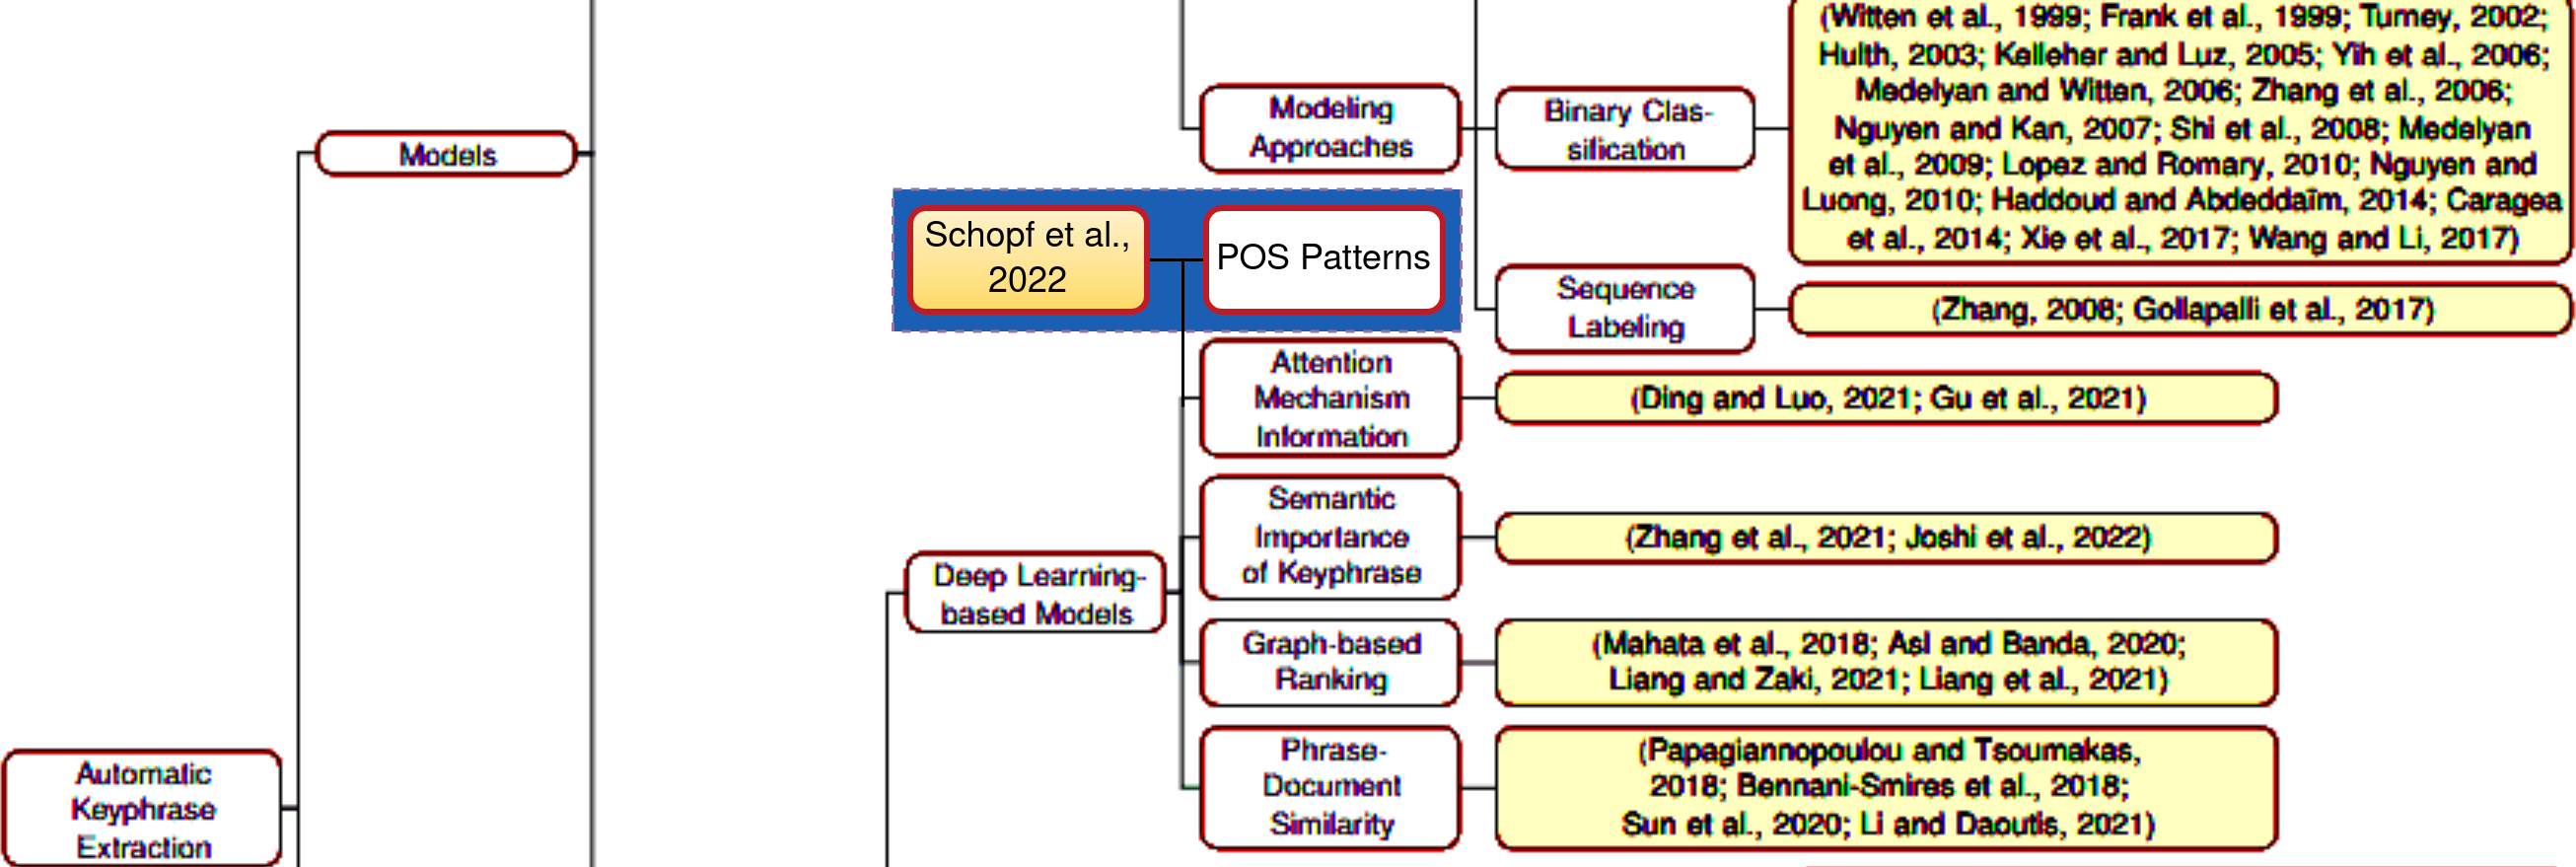
\includegraphics[width=110mm,scale=0.5]{pic/sota_lm_adapte.png}
    \caption{Extrait de l'état de l'art sur l'extraction des mots-clés, adapté de \citet{xie2023}}
    \label{fig:enter-label}
\end{figure}
\notecite{schopf2022}
\end{frame}

\begin{frame}{Fonctionnement de la méthode \textit{PatternRank}}
%\begin{itemize}
%\item extraction des phrases-clés non-supervisée
%\item exploite des modèles de langues pré-entraînés + parties du discours
%\end{itemize}
\begin{enumerate}
\item entrée : un seul document texte tokenisé
\item étiquetage des tokens avec les balises POS
\item sélection des tokens correspondant au modèle POS défini comme phrases-clés candidates
\item génération des plongements du document et des phrases-clés candidates par un modèle de langue
\item calcul des similarités cosinus entre les plongements du document et des phrases-clés candidates + classement des phrases-clés
\item extraction des \textit{N} phrases-clés les plus représentatives
\end{enumerate}
\begin{figure}
    \centering
    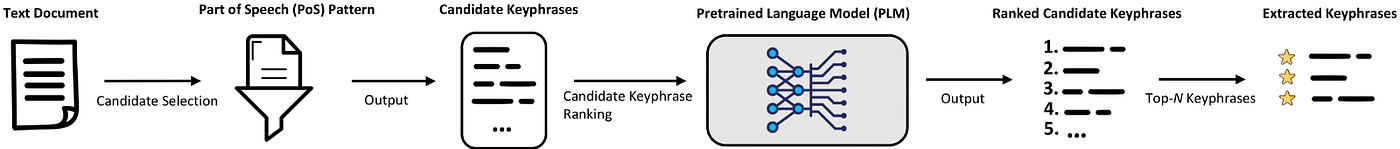
\includegraphics[width=110mm,scale=0.5]{pic/patternrank_workflow.png}
    \caption{\textit{Workflow} de la méthode \textit{PatternRank}.}
    \label{fig:enter-label}
\end{figure}
\end{frame}
%\section[\textit{PatternRank}]{Méthode \textit{PatternRank}}
\begin{frame}{\texttt{keybert} amélioré -- \textit{PatternRank}}
\onslide<+->{Key\textsc{BERT} + Keyphrase-Vectorizers = \textit{\textbf{PatternRank}} \hfill {\small\citep{schopf2022}}}
\begin{itemize}[<+->]
\item extraction des phrases-clés les plus similaires à un document
\item préservation de leur grammaticalité grâce aux motifs POS
\end{itemize}
\begin{figure}
    \centering
    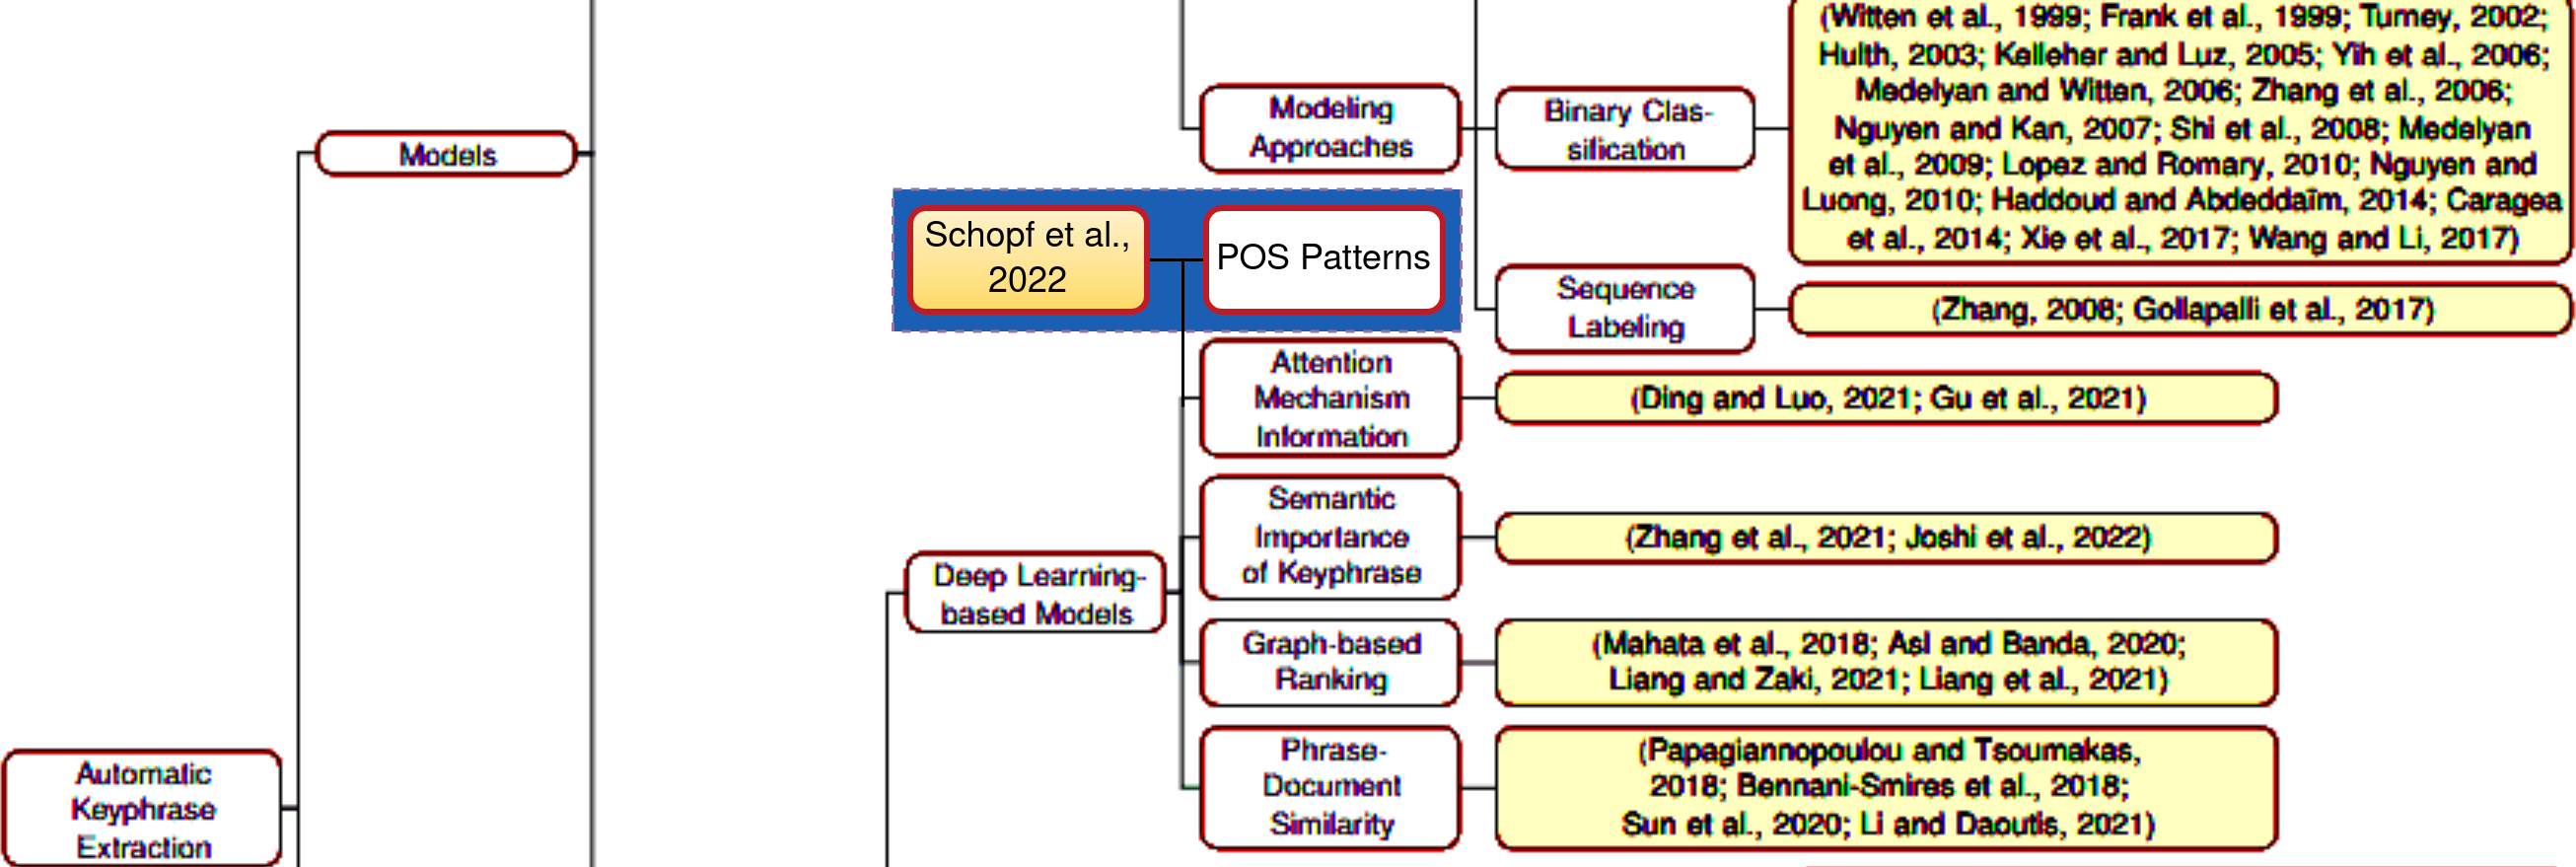
\includegraphics[width=110mm,scale=0.5]{pic/sota_lm_adapte.png}
    \caption{Extrait de l'état de l'art sur l'extraction des mots-clés, adapté de \citet{xie2023}}
    \label{fig:enter-label}
\end{figure}
\notecite{schopf2022}
\end{frame}

\begin{frame}{Fonctionnement de la méthode \textit{PatternRank}}
%\begin{itemize}
%\item extraction des phrases-clés non-supervisée
%\item exploite des modèles de langues pré-entraînés + parties du discours
%\end{itemize}
\begin{enumerate}[<+->]
\item entrée : un seul document texte tokenisé
\item étiquetage des tokens avec les balises POS
\item sélection des phrases-clés candidates correspondant au modèle POS 
\item génération des plongements du document et des phrases-clés candidates par un modèle de langue
\item calcul des similarités cosinus entre les plongements du document et des phrases-clés candidates + classement des phrases-clés
\item extraction des \textit{N} phrases-clés les plus représentatives
\end{enumerate}
\begin{figure}
    \centering
    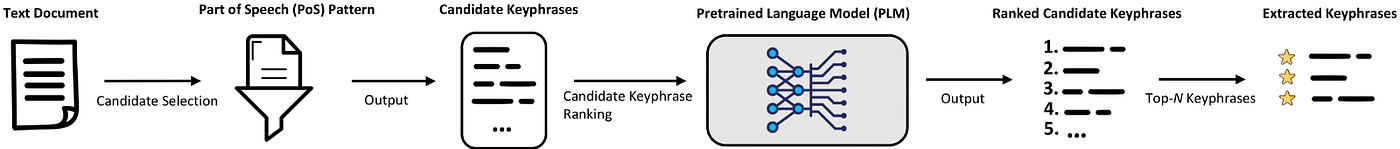
\includegraphics[width=110mm,scale=0.5]{pic/patternrank_workflow.png}
    \caption{\textit{Workflow} de la méthode \textit{PatternRank} \citep{schopf2022}.}
    \label{fig:enter-label}
\end{figure}
\end{frame}

\begin{frame}{Liste des phrases-clés avec \texttt{keyphrase-vectorizers}}
\begin{table}
\begin{tabular}{l|r}
\small
\rowcolor[HTML]{FFCCC9} 
\textsc{\textbf{Phrase-clé}} & \cellcolor[HTML]{DAE8FC}\textsc{\textbf{Score}} \\ \hline
paroi épaissie & 0.9276 \\
histologie fine & 0.9193 \\
tissu gingival & 0.9179 \\
21c leçon & 0.9162 \\
travaux récents & 0.9152 \\
entrecroisement dos pyramides & 0.9145 \\
érysipèle périodique annuel & 0.9135 \\
cicatriciel & 0.9118 \\
fibromes & 0.9109 \\
affeclions & 0.9091
\end{tabular}
\caption{Liste des dix phrases-clés les plus pertinentes selon \texttt{keyphrase-vectorizers}.}
\end{table}
\end{frame}

\begin{frame}{Utilisation des librairies \texttt{keybert} et \texttt{keyphrase-vectorizers}}
Ressources en ligne : \pause
\begin{itemize}[<+->]
\item \href{https://colab.research.google.com/drive/1sBJP-lJcKZPgIqWzFRNfrBn3domuy1tP?usp=sharing}{Lien Google Colab}\\
pré-requis :
\begin{itemize}[<+->]
\item bonne connexion Internet
\item mémoire RAM suffisante
\end{itemize}
\item \href{https://github.com/ljpetkovic/Charcot\_KeyBERT\_Keyphrase-Vectorizers?tab=readme-ov-file}{Dépôt GitHub}
\end{itemize}

\end{frame}

\begin{frame}{Passage à l'échelle}
Pour traiter de grands corpus, il existe la possibilité de demander l'accès à la plateforme technologique \href{https://sacado.sorbonne-universite.fr/}{\textsc{MeSU}}, hébergée par \textsc{SACADO} (Service d’Aide au Calcul et à l’Analyse de Données).\pause
\bigskip

Elle est composée d’un supercalculateur, d’un environnement de virtualisation et d’un système de stockage de données.
\end{frame}





% \appendix

\begin{frame}[allowframebreaks]{Références}
\printbibliography

\end{frame}

\end{document}